\chapter{Preliminares}

En esta sección introductoria se abordarán algunas propiedades fundamentales de los números reales, cuyo estudio resulta esencial para la comprensión rigurosa de los principios del cálculo. A partir del análisis del concepto de número real, del plano cartesiano y de otras nociones preliminares, se pretende establecer una base conceptual sólida que facilite la transición hacia el estudio formal del cálculo diferencial e integral, estructurado desde la noción de función.

\section{Números reales}

Uno de los conceptos más fundamentales en las matemáticas es el de número, cuya noción se remonta a la antigüedad y cuya generalización se ha desarrollado a lo largo de la historia. La estructura numérica básica se origina en el conjunto de los \textit{números naturales}, que posteriormente se amplió al incorporar los números negativos, dando lugar a los \textit{números enteros}. Más adelante, al considerar la posibilidad de expresar un número como una fracción de la forma $\dfrac{a}{b}$, donde $a$ y $b$ son enteros con $b \neq 0$, surge el conjunto de los \textit{números racionales}, los cuales pueden representarse mediante expresiones decimales finitas o periódicas infinitas. 

Desde la época de los pitagóricos, se reconoce la existencia de los \textit{números irracionales}, aquellos que no pueden expresarse como cociente de dos números enteros; un ejemplo clásico es $\sqrt{2}$. La unión de los números racionales e irracionales da origen al conjunto de los \textbf{números reales}, que constituirá el objeto principal de estudio en esta sección.

El descubrimiento de los números irracionales, atribuido a la escuela pitagórica en la antigua Grecia (siglo V a.\,C.), representó una crisis intelectual para la concepción aritmética de la época, pues reveló la existencia de magnitudes inconmensurables. Este hallazgo marcó un punto de inflexión en el pensamiento matemático, impulsando el desarrollo posterior de la teoría de los números y la formalización del concepto de continuidad numérica.

A continuación se presentan algunas propiedades fundamentales de los números reales, cuya comprensión resulta esencial para el estudio riguroso del análisis matemático.

\subsection{Propiedades de los números reales}

\begin{theorem}[Propiedad de tricotomía]
El conjunto de los números reales forma un cuerpo ordenado. En particular, dados $x$ y $y$ números reales, existe una y solo una de las siguientes relaciones: $x < y$, $x = y$ o $x > y.$
\end{theorem}

Los números reales pueden representarse sobre la \textbf{recta numérica infinita} (o \textit{eje real}) de acuerdo con la siguiente convención (figura \ref{rectanumerica}): se define un punto $O$, denominado \textit{origen}, que representa al número $0$; una flecha orientada hacia la derecha indica la dirección positiva, mientras que una flecha orientada hacia la izquierda representa los valores negativos. 

Por ejemplo, si un número $x_1$ es positivo, se ubica en la recta como un punto a la derecha del origen, a una distancia proporcional a su valor. De manera análoga, si un número $x_2$ es negativo, se representa como un punto a la izquierda del origen, también a una distancia proporcional a $|x_2|$. 

\begin{figure}[H] \label{rectanumerica}



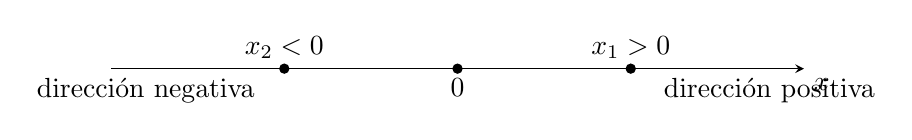
\begin{tikzpicture}[>=stealth, scale=1.1]
  % Eje real
  \draw[->] (-4,0) -- (4,0) node[below right] {$x$};
  
  % Origen
  \draw[fill] (0,0) circle (1.5pt) node[below] {$0$};
  
  % Marca y etiqueta de un número positivo x_1
  \draw[fill] (2,0) circle (1.5pt) node[above] {$x_1>0$};
  
  % Marca y etiqueta de un número negativo x_2
  \draw[fill] (-2,0) circle (1.5pt) node[above] {$x_2<0$};
  
  % Indicaciones de direcciones positiva y negativa
  \node[below] at (3.6,0) {dirección positiva};
  \node[below] at (-3.6,0) {dirección negativa};
\end{tikzpicture}
\caption{Recta numérica o eje real}

\end{figure}

Existe así una correspondencia biunívoca entre los números reales y los puntos de la recta numérica: a cada número real le corresponde un punto único, y a cada punto, un número real. Además, debido a una propiedad denominada \textbf{completitud de los números reales} —cuyo tratamiento formal excede los alcances de este curso—, se cumple que entre dos números reales cualesquiera siempre es posible encontrar otros números, sean racionales o irracionales. Esta idea se resume en el siguiente teorema clásico.

\begin{theorem}
Para todo número irracional $\alpha$, existen infinitos números racionales que lo aproximan con cualquier grado deseado de precisión.
\begin{proof}
Sea $\alpha > 0$ un número irracional. Queremos calcular una aproximación con un error menor que $\dfrac{1}{n}$. Note que, para cualquier $\alpha$, existe un número entero $N$ tal que $N < \alpha < N + 1$. Si se divide el segmento comprendido entre $N$ y $N + 1$ en $n$ partes iguales, entonces $\alpha$ se encontrará entre $N + \dfrac{m}{n}$ y $N + \dfrac{m + 1}{n}$ para algún entero $m$. La diferencia entre ambos extremos es $\dfrac{1}{n}$, de modo que se puede alcanzar cualquier precisión deseada disminuyendo el valor de $\dfrac{1}{n}$.
\end{proof}
\end{theorem}

\begin{example}
El número irracional $\sqrt{2}$ puede aproximarse de la siguiente manera:
\begin{align*}
1.4 &< \sqrt{2} < 1.5,\\
1.41 &< \sqrt{2} < 1.42,\\
1.414 &< \sqrt{2} < 1.415,
\end{align*}
según precisiones de $\dfrac{1}{10}$, $\dfrac{1}{100}$ y $\dfrac{1}{1000}$, respectivamente.
\end{example}

\subsection{Valor absoluto de los números reales}

\begin{definition}[Valor absoluto]
El \textbf{valor absoluto} (o módulo) de un número real $x$, denotado por $|x|$, se define como:
\begin{align*}
|x| &= x & \text{si } x \geq 0,\\
|x| &= -x & \text{si } x < 0.
\end{align*}
Por esta definición, $|x|$ representa siempre un número real no negativo ($|x| \geq 0$) y mide la distancia de $x$ al origen en la recta numérica.
\end{definition}

\begin{example}
Para $x = 2$, se tiene $|2| = 2 \geq 0$. Para $x = -3$, se verifica $|-3| = 3 > 0$. En ambos casos, el valor absoluto produce un número no negativo.
\end{example}

A continuación se enuncian las propiedades fundamentales del valor absoluto:

\begin{theorem}[Propiedades del valor absoluto]
Dados $x, y \in \mathbb{R}$, se cumplen las siguientes propiedades:
\begin{enumerate}
\item $|x + y| \leq |x| + |y|$ (Desigualdad triangular).
\item $|x - y| \geq \bigl||x| - |y|\bigr|$ (Segunda desigualdad triangular).
\item $|xy| = |x| \cdot |y|$ para todo $x, y \in \mathbb{R}$.
\item $\left|\dfrac{x}{y}\right| = \dfrac{|x|}{|y|}$ siempre que $y \neq 0$.
\end{enumerate}
\end{theorem}

\begin{proof}


\begin{enumerate}
\item \textbf{Caso $1$:} $x + y \geq 0$. Entonces $|x + y| = x + y \leq |x| + |y|$, pues $|x| \geq x$ y $|y| \geq y$.

\textbf{Caso $2$:} $x + y < 0$. Entonces $|x + y| = -(x + y) = (-x) + (-y) \leq |x| + |y|$, ya que $|x| \geq -x$ y $|y| \geq -y$.

\item Sea $z = x - y$. Entonces $x = y + z$, y por la desigualdad triangular:
\[
|x| = |y + z| \leq |y| + |z| = |y| + |x - y|.
\]
Restando $|y|$ de ambos lados: $
|x| - |y| \leq |x - y|.$ 

Dado que la desigualdad es simétrica, también se tiene $|y| - |x| \leq |x - y|$, lo que equivale a:
\[
|x - y| \geq \bigl||x| - |y|\bigr|.
\]

Las propiedades $3$ y $4$ se siguen directamente de la definición del valor absoluto.
\end{enumerate}
\end{proof}



\subsection{Magnitudes variables y constantes e intervalos de variación}

Las \textbf{magnitudes variables}, tales como el tiempo, longitud, área, volumen, masa, velocidad y temperatura, obtienen sus valores mediante el hábito de la medición y se presentan en sucesión constante. Para el caso del movimiento uniforme, podemos observar el desplazamiento de un punto a lo largo del tiempo.

Por contraste, las \textbf{magnitudes constantes} son aquellas que no sufren variación; una magnitud variable cuyo valor permanece invariable se denomina constante. La distinción entre magnitudes variables y constantes resulta fundamental en el análisis matemático. De esto, por ejemplo $\pi\approx 3.14159$ es una constante mientras $t$ vista como el tiempo es variable.

Una magnitud variable puede tomar diferentes valores numéricos. Se considera el problema de la temperatura del agua al calentarla en condiciones normales, variará desde $15^\circ$C hasta el punto de ebullición: $100^\circ$C.

\begin{figure}[H]
\centering
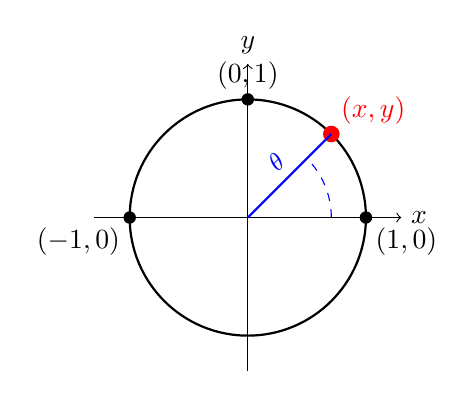
\begin{tikzpicture}[scale=1.5]
  % Círculo unitario
  \draw[thick] (0,0) circle (1cm);
  % Ejes
  \draw[->] (-1.3,0) -- (1.3,0) node[right] {$x$};
  \draw[->] (0,-1.3) -- (0,1.3) node[above] {$y$};
  % Puntos cardinales
  \fill (-1,0) circle (1.5pt) node[below left] {$(-1,0)$};
  \fill (1,0) circle (1.5pt) node[below right] {$(1,0)$};
  \fill (0,1) circle (1.5pt) node[above] {$(0,1)$};
  % Punto genérico (x,y) en el primer cuadrante
  \fill[red] (0.707,0.707) circle (2pt) node[above right] {$(x,y)$};
  % Ángulo theta desde origen al punto (x,y)
  \draw[blue, thick] (0,0) -- (0.707,0.707) node[midway, sloped, above, font=\small] {$\theta$};
  % Arco para enfatizar el ángulo
  \draw[blue, dashed] (0.707,0) arc (0:45:0.707cm);
\end{tikzpicture}
\caption{Representación trigonométrica en el círculo unitario: $x = \cos\theta$, $y = \sin\theta$, donde $(x,y)$ satisface $x^2 + y^2 = 1$}
\label{fig:circulo}
\end{figure}


La variable $z = \cos\theta$ puede tomar todos los valores comprendidos entre $-1$ y $+1$. El conjunto de todos los valores posibles que puede tomar la variable independiente $\theta$ se denomina \textbf{campo de variación} de la variable independiente, el cual determina el conjunto de valores posibles de la función dependiente. 

Por ejemplo, en la función $z = \cos\theta$, el \textbf{campo de variación} de $z$ es el intervalo cerrado $[-1,1]$. Posteriormente, este concepto se denominará formalmente \textit{rango} (o \textit{imagen}) de una función.

Observe que hemos introducido la notación de intervalo $[-1,1]$. Esta notación se define de la siguiente manera:


\begin{definition}[Intervalos]
Un \textbf{intervalo} es el conjunto de valores numéricos $x \in \mathbb{R}$ comprendidos entre dos números reales dados $a$ y $b$ ($a < b$). Los intervalos se clasifican según los extremos incluidos:

\begin{itemize}
\item \textbf{Intervalo abierto}: $(a,b) = \{ x \in \mathbb{R} \mid a < x < b \}$. \textit{No se incluyen los extremos $a$ ni $b$.}
\item \textbf{Intervalo cerrado}: $[a,b] = \{ x \in \mathbb{R} \mid a \leq x \leq b \}$. \textit{Se incluyen ambos extremos.}
\item \textbf{Intervalos semicerrados (o semiabiertos)}:
  \begin{itemize}
  \item $(a,b] = \{ x \in \mathbb{R} \mid a < x \leq b \}$
  \item $[a,b) = \{ x \in \mathbb{R} \mid a \leq x < b \}$
  \end{itemize}
\item \textbf{Intervalos infinitos}:
  \begin{itemize}
  \item $(-\infty,c) = \{ x \in \mathbb{R} \mid x < c \}$
  \item $(c,+\infty) = \{ x \in \mathbb{R} \mid x > c \}$
  \item $(-\infty,+\infty) = \mathbb{R}$
  \end{itemize}
\end{itemize}

Existen combinaciones adicionales de estas definiciones, como por ejemplo $(-\infty,b]$, que se interpretan de manera análoga.
\end{definition}

\begin{example}
Ejemplos de intervalos: $(-1,1)$, $[-2,3)$, $(0,+\infty)$, $\mathbb{R} = (-\infty,+\infty)$.
\end{example}

Las definiciones de intervalos abiertos y cerrados se utilizan para múltiples aspectos de las funciones. Gráficamente se considera el concepto de vecindad, que está representada por un centro y un radio, el cual resulta ser un intervalo: 

\begin{figure}[H]
\centering
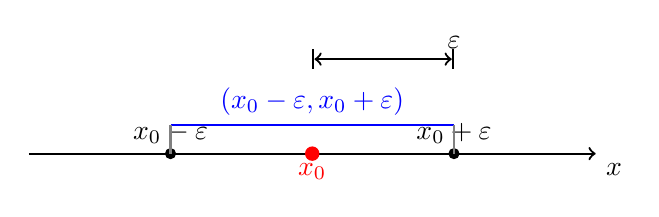
\begin{tikzpicture}[scale=1.2]
  % Eje real
  \draw[thick, ->] (-3,0) -- (3,0) node[below right] {$x$};
  
  % Límites de la vecindad (puntos extremos)
  \filldraw (-1.5,0) circle (1.5pt) node[above] {$x_0-\varepsilon$};
  \filldraw (1.5,0) circle (1.5pt) node[above] {$x_0+\varepsilon$};
  
  % Centro x_0
  \filldraw[red] (0,0) circle (2pt) node[below] {$x_0$};
  
  % Línea horizontal superior para representar el intervalo abierto
  \draw[thick, blue] (-1.5,0.3) -- (1.5,0.3);
  
  % Flechas verticales en los extremos para mostrar apertura
  \draw[thick, gray] (-1.5,0) -- (-1.5,0.3);
  \draw[thick, gray] (1.5,0) -- (1.5,0.3);
  
  % Doble flecha para radio \varepsilon (simétrica)
  \draw[thick, |<->|] (0,1) -- (1.5,1) node[above] {$\varepsilon$};
  
  % Etiqueta opcional para el intervalo
  \node[above, blue] at (0,0.3) {$(x_0 - \varepsilon, x_0 + \varepsilon)$};
\end{tikzpicture}
\caption{Intervalo abierto $(x_0 - \varepsilon, x_0 + \varepsilon)$ representado como línea centrada en $x_0$ de radio $\varepsilon$ en el eje real.}
\label{fig:vecindad}
\end{figure}





\begin{definition}[Vecindad]
Dados un número real $x_0 \in \mathbb{R}$ y un número positivo $\varepsilon > 0$, el conjunto $(x_0 - \varepsilon, x_0 + \varepsilon)$ se denomina \textbf{vecindad} de $x_0$ de \textbf{radio} $\varepsilon$, o simplemente vecindad de radio $\varepsilon$ centrada en $x_0$. En este caso, el punto $x_0$ se llama \textbf{centro} de la vecindad, y la magnitud $\dfrac{\varepsilon}{2}$ denomina \textbf{radio de la vecindad}. La Figura \ref{fig:vecindad} representa la vecindad $(x_0 - \varepsilon, x_0 + \varepsilon)$ del punto $x_0$, cuyo radio es $\varepsilon$.
\end{definition}

\subsection{Problemas propuestos}

Siga estos pasos ordenados para resolver los problemas algebraicos. Estos pasos son útiles tanto para su resolución manual como para generar prompts efectivos con inteligencia artificial.

\textbf{PROCESO SISTEMÁTICO DE RESOLUCIÓN}

\begin{enumerate}
\item \textbf{ANÁLISIS INICIAL}
   \begin{itemize}
   \item Lea todo el problema cuidadosamente.
   \item Identifique: ¿Qué datos se dan? ¿Qué se pide?
   \item Clasifique el problema: ecuación, desigualdad, simplificación, o aplicado.
   \end{itemize}

\item \textbf{PLAN DE SOLUCIÓN}
   \begin{itemize}
   \item Liste las técnicas necesarias: factorización, valor absoluto, despeje, etc.
   \item Si es aplicado, asigne variables a las incógnitas.
   \end{itemize}

\item \textbf{EJECUCIÓN ALGEBRAICA}
   \begin{itemize}
   \item Organice la ecuación/desigualdad claramente.
   \item Identifique simplificaciones: fracciones, factorización, radicales.
   \item Realice operaciones paso a paso, explicando cada acción:
     \begin{itemize}
     \item ``Multiplico por $x-2\neq 0$ para eliminar denominador''
     \item ``Factorizo numerador: $x^2-4=(x-2)(x+2)$''
     \end{itemize}
   \end{itemize}

\item \textbf{VALIDACIÓN DE SOLUCIONES}
   \begin{itemize}
   \item Verifique soluciones extraviadas (raíces, valor absoluto).
   \item Determine dominio: denominadores ≠0, radicales ≥0.
   \item Sustituya en la expresión original.
   \end{itemize}

\item \textbf{PRESENTACIÓN FINAL}
   \begin{itemize}
   \item Expresión simplificada o intervalo solución.
   \item Dominio completo.
   \item Contexto físico (si aplica).
   \end{itemize}
\end{enumerate}



\begin{prob}
Encuentre los valores de $x \in \mathbb{R}$ que resuelven las siguientes ecuaciones o desigualdades. Expresa las soluciones en notación de intervalo cuando corresponda y represente gráficamente cada conjunto solución como vecindad abierta en el eje real (incluya la figura con centro y radio $\varepsilon$ apropiados).

\begin{multicols}{2}
\begin{enumerate}

% I. Ecuaciones Racionales y Radicales (5)
\item \(\displaystyle \frac{3x + 1}{5x + 7} = \frac{6x + 11}{10x - 3}\)
\item \(\displaystyle 2 - \frac{1}{x} = 1 + \frac{3}{x}\)
\item \(\displaystyle \frac{2}{x+5} = \frac{3}{2x + 1} - \frac{5}{6x + 3}\)
\item \(\displaystyle \frac{4}{x - 5} - \frac{2}{x + 4} = \frac{3}{2x - 4}\)
\item \(\displaystyle \frac{1}{\sqrt{x}} = 3 - \frac{1 - 3\sqrt{x}}{\sqrt{x}}\)

% II. Ecuaciones Cuadráticas y Polinómicas (5)
\item \(2x^{2} + 7x - 15 = 0\)
\item \((x - 2)(x + 1) - 6 = 0\)
\item \(4x^{2} - 37x^{2} + 75 = 0\)
\item \(x^{2} - 2x - 15 = 0\)
\item \(20x^{2} + 8x^{2} - 55x - 22 = 0\)

% III. Operaciones Algebraicas con Fracciones (5)
\item \(\displaystyle \frac{6xy^{2}}{7} \times \frac{21x^{2}}{y} \div \frac{32xy^{2}}{91}\)
\item \(\displaystyle \frac{12p^{2}q^{2}}{5} \times \frac{15}{4pq} \div 3\)
\item \(\displaystyle \frac{3}{pq} \times \frac{4p}{p+1}\)
\item \(\displaystyle \frac{x^{2} - x - 6}{2xy} \times \frac{2x^{2}y}{x^{2} - 9}\)
\item \(\frac{4}{\sqrt{2} - 1} + \frac{4 + \sqrt{3}}{\sqrt{2} - 3}\)

% IV. Desigualdades Lineales y Polinómicas (5)
\item \(3x - 2 > 12\)
\item \(2x + 5 \leq 8\)
\item \(-2 - 3x \geq 2\)
\item \(3 - 5x < 11\)
\item \(2x + 5 < 6x - 7\)

% V. Ecuaciones y Desigualdades con Valor Absoluto (5)
\item \(|4x - 1| = 7\)
\item \(|2x + 1| + 1 = 15\)
\item \(\left| \frac{2 - 3x}{5} \right| = 2\)
\item \(\left| \frac{2x + 5}{3} \right| < 1\)
\item \(\frac{3}{|5 - 2x|} < 2\)

% VI. Desigualdades Racionales y Polinómicas (5)
\item \(\displaystyle \frac{x^{2}(x + 2)}{x + 2(x + 1)} \leq 0\)
\item \(\displaystyle \frac{(x^{2} + 1)(x - 3)}{x^{2} - 9} \geq 0\)
\item \(\displaystyle \frac{x^{2} - x}{x^{2} + 2x} \leq 0\)
\item \(\displaystyle \frac{(x + 3)(2 - x)}{(x + 4)(x^{2} - 4)} \leq 0\)
\item \(\displaystyle \frac{x - 2}{3x - 10} \geq 0\)

\end{enumerate}
\end{multicols}
\end{prob}


